% // TODO: Pasar esto a limpio
% Una geometría es el estudio cuantitativo de las formas y su evolución para ciertas figuras de un espacio
% 
%         Espacio ambiente                     | Figuras                                          | Soporte Matemático                                                                        |
%         -------------------------------------|--------------------------------------------------|-------------------------------------------------------------------------------------------|
% Gª I:   Espacio vectorial                    | Subespacios vectoriales: rectas, planos, ...     | Espacio vectorial, intersecciones y sumas                                                 |
% Gª II:  Espacio vect euclideo                | Subespacios vectoriales: rectas, planos, ...     | Espacio vectorial con una métrica, intersecciones, sumas, perpendicularidad, medir ángulos|
% Gª III: Espacio afin euclideo                | Subespacios afines: puntos, rectas, planos, ...  | Espacio afin con una métrica en el esp. vect. asociado                                    |
%                                              | cónicas y cuádricas                              | intersecciones, sumas, perpendicularidad, medir ángulos, medir distancias                 |
% Tª I:   Ninguno o un e.t.                    | Subespacios topológicos                          | Topología en un conjunto, determinar homeomorfismos                                       |
% Tª II:  Ninguno o un e.t.                    | Subespacios topológicos                          | Topología en un conjunto, determinar homeomorfismos, teoría de grupos                     |
% CyS:    Curvas en R² o R³, Superficies en R³ | Curvas en R² o R³, Superficies en R³             | Todas las anteriores + análisis                                                           |
% 
% En Gª I y II los soportes matemáticos tienen que ver con polinomios de primer grado homogéneos
% En Gª III son polinomios de primer y segundo grado, se va a la geometría algebraica
% 
% CyS / Introducción a la Geometría Diferencial (Análisis Geométrico)
% 
%
% Cronológicamente:
% GII y GIII, puntos, rectas, planos, ...
% CyS, curvas y superficies, sigo XVII
% Topologías, siglo XX
% GI, espacio vectorial
%
%
% CyS:
% epicicloide: curva que describe un punto de una rueda al girar
% 
% Protagonistas:
% siglo 17: Leibniz, Newton
% siglo 18: Euler, Monge
% siglo 19: Frenet, Senet, Escuela Francesa, Cauchy
% siglo 20: Darboux, Cartan

\chapter{Curvas en el plano y en el espacio}
\section{Definición. Curva regular. Longitud de arco}
\begin{definicion}
    Una \textbf{curva} en el espacio es una aplicación diferenciable $\alpha:I\to \mathbb{R}^3$ donde $I\subseteq \mathbb{R}$ es un intervalo abierto.\\

    \noindent
    Normalmente, si queremos señalar explícitamente las componentes de $\alpha$, escribiremos:
    \begin{equation*}
        \alpha(t) = (x(t), y(t), z(t))
    \end{equation*}
    En realidad, a un geómetra solo le interesa la llamada ``traza de la curva'':
    \begin{equation*}
        \tr \alpha = \im \alpha = \alpha(I)
    \end{equation*}
\end{definicion}

\begin{ejemplo}
    Sean $a\in \mathbb{R}^3$, $v\in \mathbb{R}^3$, definimos $\alpha:\mathbb{R}\to \mathbb{R}^3$ dada por:
    \begin{equation*}
        \alpha(t) = a + tv 
    \end{equation*}
    En dicho caso:
    \begin{equation*}
        \tr \alpha = \left\{\begin{array}{ll}
            \{a\} & \text{si\ } v=0 \\
             R_{a,v} & \text{si\ } v\neq 0
        \end{array}\right. 
    \end{equation*}
    donde denotamos por $R_{a,v}$ a la única recta que pasar por $a$ y con dirección $v$:
    \begin{equation*}
        R_{a,v} = a + \langle v \rangle 
    \end{equation*}

    \begin{figure}[H]
        \centering
        \begin{tikzpicture}
        \draw (-2,0) -- (2,0);
        \draw[-Stealth] (0,0) -- (1,0);
        \fill (0,0) circle(2pt) node[below] {$a$};
        \fill (0.5, 0) node[above] {$v$};
        \fill (-1, 0) node[above] {$R_{a,v}$};
        \end{tikzpicture}
    \end{figure}
\end{ejemplo}

\begin{definicion}
    Una curva $\alpha:I\to \mathbb{R}^3$ se llama ``\textbf{plana}'' si existe un plano $P\subset \mathbb{R}^3$ tal que $\tr \alpha \subset P$.\\

    \noindent
    Como $P$ y $P(z=0)$ son equivalentes salvo un movimiento rígido\footnote{Es decir, una aplicación afín que conserve longitudes y ángulos.} de $\mathbb{R}^3$, podemos considerar que la curva $\alpha$ está definida como $\alpha:I\to P(z=0)\subset \mathbb{R}^3$, cuyas componentes son:
    \begin{equation*}
        \alpha(t) = (x(t), y(t), 0) \equiv (x(t), y(t))
    \end{equation*}
    De esta forma, podemos abstraernos y pensar que una curva plana es una aplicación diferenciable $\alpha:I\to \mathbb{R}^2$.
\end{definicion}~\\

\noindent
En los libros es común llamar a estar curvas ``parametrizadas'' y ``diferenciables''. En nuestra definición imponemos que una curva ha de ser diferenciable, y el adjetivo parametrizada se debe a la dependencia de la variable independiente.

% // TODO: Buscar software para dibujar curvas en R³.

\begin{ejemplo}
    Varios ejemplos de curvas:
    \begin{enumerate}
        \item Extrapolando el ejemplo anterior:
            \begin{equation*}
                \alpha(t) = a + tv
            \end{equation*}
            para $a\in \mathbb{R}^2, v\in \mathbb{R}^2$ y $\alpha'(t) = v$. Se trata de un Movimiento Rectilíneo Uniforme. Ahora, vemos que $\alpha''(t) = 0$, no hay aceleración ninguna.
        \item Tomando $a\in \mathbb{R}^2$ y $v\in \mathbb{R}^2\setminus \{0\}$, consideramos $\beta:\mathbb{R}\to \mathbb{R}^2$ dada por:
            \begin{equation*}
                \beta(t) = a+t^2v
            \end{equation*}
            Observamos ahora que tenemos $\tr \beta\subset \tr \alpha$, y la traza de esta curva es la semirrecta de extremo $a$ y dirección $v$:
            \begin{equation*}
                \tr \beta = R_0^+(a,v) 
            \end{equation*}
            \begin{figure}[H]
                \centering
                \begin{tikzpicture}
                \draw (0,0) -- (3,0);
                \draw[-Stealth] (0,0) -- (1,0);
                \fill (0,0) circle(2pt) node[below] {$a$};
                \fill (0.5,0) node[above] {$v$};
                \fill (2,0) node[above] {$\tr \beta$};
                \end{tikzpicture}
            \end{figure}

            Desde el punto de vista físico, muy en el pasado (límite en $-\infty$) estábamos muy alejados del punto $a$. A medida que nos vamos acercando a tiempo $0$ nos vamos acercando al punto $a$ con una velocidad de módulo decreciente que se hace cero cuando alcanzamos el instante $t=0$ y que luego aumenta posteriormente mientras el móvil se aleja del punto $a$ en la dirección en la que vino.

            Vemos que tenemos una velocidad $\beta'(t) = 2tv$, así como una aceleración $\beta''(t) = 2v$, que es constante, por lo que estamos ante un Movimiento Rectilíneo Uniformemente Acelerado.

            El punto $a$ (que se alcanza en $t=0$) es un punto extraño, es el único punto de $\tr \beta$ en su frontera. Además, podemos observar que en dicho punto tenemos $\beta'(0) = 0$.
    \end{enumerate}
\end{ejemplo}

\begin{ejercicio} 
    Estudiar $\gamma(t) = a+t^3 v$, con $a\in \mathbb{R}^2$ y $v\in \mathbb{R}^2\setminus \{0\}$.

    \noindent
    Es claro que $\tr \gamma = R_{a,v} = \tr \alpha$. En este caso tenemos:
    \begin{equation*}
        \gamma'(t) = 3t^2v, \qquad \gamma''(t) = 6tv
    \end{equation*}
    Vemos que la velocidad es siempre positiva y en este caso la aceleración no es constante: es decreciente cuando $t<0$ y es creciente cuando $t>0$, simula la situación en la que un móvil se acerca al punto $a$ frenando cada vez más fuerte y a medida que pasa el punto $a$ comienza a acelerar cada vez más rápido.
\end{ejercicio}

\begin{ejemplo}
    Siguiendo con más ejemplos:
    \begin{enumerate}
        \setcounter{enumi}{2}
        \item Consideramos ahora $\delta:\mathbb{R}\to \mathbb{R}^2$ dada por:
            \begin{equation*}
                \delta(t) = (t^3-4t, t^2-4)
            \end{equation*}
            Para pensar la curva primero analizamos dónde esta corta el eje $x$:
            \begin{equation*}
                t^2-4 = 0 \Longleftrightarrow t = \pm 2
            \end{equation*}
            En dichas abscisas, la curva toma la ordenada:
            \begin{equation*}
                \delta(-2) = 0 = \delta(2)
            \end{equation*}
            Por lo que en ambos instantes de tiempo la curva pasa por el origen. Si estudiamos el corte con el eje $y$ vemos que tiene 3 puntos de corte, dos de ellos ya los conocemos y el que falta es en el instante $t=0$; donde alcanza una ordenada de $-4$. Teniendo en cuenta también los límites en $-\infty$ y en $+\infty$ podemos finalmente deducir que la curva será algo del estilo:
            \ifshowfigures
            \begin{figure}[H]
                \centering
                \begin{tikzpicture}[scale=0.8]
                    % Ejes
                    \draw[-Stealth] (-5,0) -- (5,0) node[right] {$x$};
                    \draw[-Stealth] (0,-4.5) -- (0,3) node[above] {$y$};

                    % Curva parametrizada
                    \draw[domain=-2.5:2.5, samples=200, smooth, thick, blue] 
                        plot ({\x*\x*\x - 4*\x}, {\x*\x - 4});
                \end{tikzpicture}
            \end{figure}
            \fi

            \noindent
            Vemos que esta curva tiene autointersecciones, por lo que las curvas no tienen por qué ser inyectivas.

        \item Si consideramos $\varepsilon:\mathbb{R}\to \mathbb{R}^2$ dada por $\varepsilon(t) = (t^3,t^2)$.

            Su velocidad es $\varepsilon'(t) = (3t^2, 2t)$, que se anula en el origen. Observamos que en el dibujo de la traza vemos un pico.

            Aunque $\varepsilon$ sea diferenciable, $\tr \varepsilon$ tiene ``picos''. Observamos además que $\im \varepsilon$ es la gráfica de la aplicación\footnote{Lo hemos obtenido igualando $x=t^3$, $y=t^2$, despejando $t$ de la primera e igualando en la segunda.} $y=x^{\nicefrac{2}{3}}$. Esta función no es derivable en el origen, a pesar de que la curva sí lo sea.

            \ifshowfigures
            \begin{figure}[H]
                \centering
                \begin{tikzpicture}
                    % Ejes
                    \draw[-Stealth] (-4,0) -- (4,0) node[right] {$x$};
                    \draw[-Stealth] (0,-1) -- (0,2) node[above] {$y$};

                    % Curva parametrizada
                    \draw[domain=-1.5:1.5, samples=20, smooth, thick, blue] 
                        plot ({\x*\x*\x}, {\x*\x});
                \end{tikzpicture}
            \end{figure}
            \fi

        \item Sea $\zeta:\mathbb{R}\to \mathbb{R}^3$ dada por $\zeta(t) = a+r\left(\cos\left(\frac{t}{r}\right)e_1 + \sen\left(\frac{t}{r}\right)e_2\right)$ donde $a\in \mathbb{R}^3$, $e_1,e_2$ con $|e_1| = 1 = |e_2|$ con $\langle e_1,e_2 \rangle =0$ y $r>0$.

            Observamos que tenemos siempre:
            \begin{equation*}
                \zeta(t) \in P = a + \langle \{e_1,e_2\} \rangle \qquad \forall t\in \mathbb{R}
            \end{equation*}
            Por lo que:
            \begin{equation*}
                \im \zeta = \tr \zeta \subset P
            \end{equation*}
            Es decir, $\zeta$ es una curva plana. Además, vemos que:
            \begin{equation*}
                |\zeta(t) - a|^2 = r^2 \quad\Longrightarrow\quad |\zeta(t)-a| = r \qquad \forall t\in \mathbb{R}
            \end{equation*}
            Como $\tr \zeta$ no se puede salir del plano y equidista una cantidad $r$ de $a$, tenemos que $\tr \zeta \subset C(a,r)\subset P$.

            A esta curva la llamaremos \textbf{la\footnote{A esta la parametrizaremos siempre de la misma forma, aunque distintas parametrizaciones den la misma traza.}} circunferencia de centro $a$ y radio $r>0$ en $P$.

            Observamos que:
            \begin{equation*}
                \zeta'(t) = -\sen\left(\frac{t}{r}\right)e_1 + \cos\left(\frac{t}{r}\right)e_2 \qquad \forall t\in \mathbb{R}
            \end{equation*}
            No es constante, por lo que no es un MRU. Además vemos que $\zeta''(t)$ no es constante, por lo que tampoco es un MRUA. Sin embargo, apreciamos que $|\zeta''(t)|$ sí que es constante, así como que $|\zeta'(t)| = 1$.

            Se trata de la traza de un Movimiento Circular Uniforme.
        \item Sea $\eta:I\to \mathbb{R}^2$ con $I = \left]-1,+\infty\right[$ dada por:
            \begin{equation*}
                \eta(t) = \left(\frac{3t}{1+t^3}, \frac{3t^2}{1+t^3}\right)
            \end{equation*}
            Si pensamos en su representación, tras un poco de análisis (límite en más y menos infinito, puntos de corte con los ejes, observar que si $t>0$ siempre se encuentra en el primer cuadrante, \ldots) podemos llegar a deducir que su forma ha de ser similar a algo como:
            \ifshowfigures
            \begin{figure}[H]
            \centering
            \begin{tikzpicture}
                % Ejes
                \draw[-Stealth] (-2,0) -- (2,0) node[right] {$x$};
                \draw[-Stealth] (0,-0.5) -- (0,2) node[above] {$y$};

                % Curva parametrizada
                \draw[domain=-0.6:20, samples=100, smooth, thick, blue] 
                    plot ({3*\x/(1 + \x*\x*\x)}, {3*\x*\x/(1 + \x*\x*\x)});

                \draw[thick, blue] (0.01,0) -- (0.01,0.2);
            \end{tikzpicture}
            \end{figure}
            \fi

            \noindent
            Vemos que $\eta(0) = (0,0)$ y que $\lim_{t\to+\infty}\eta(t) = (0,0)$, pero a pesar de ello la curva no se autointerseca, ya que podemos probar que es inyectiva:

            \noindent
            Sean $u,t\in \mathbb{R}$ con $u,t>-1$ tales que $\eta(t) = \eta(u)$ tenemos entonces que:
            \begin{equation*}
                \left.\begin{array}{l}
                        \dfrac{3t}{1+t^3} = \dfrac{3u}{1+u^3} \\
                        \\
                        \dfrac{3t^2}{1+t^3} = \dfrac{3u^2}{1+u^3} 
                \end{array}\right\} \quad\Longrightarrow\quad \dfrac{3u^2}{1+u^3} = t\cdot \dfrac{3t}{1+t^3} = \dfrac{3ut}{1+u^3} 
            \end{equation*}
            Si $u\neq 0$ podemos dividir entre $u$ y concluir que $u=t$ y si $u=0$ ha de ser $t=0 =u$ para obtener $\eta(t) = \eta(u)$. Hemos probado que $\eta$ es inyectiva.

            Vemos otro hecho que hemos de tener en cuenta, y es que en este ejemplo $I$ no es homeomorfo a $\tr \eta$, puesto que si hubiera un homeomorfismo, podemos tomar cualquier entorno de $\eta(0)$ este ha de contener una bola abierta de centro $\eta(0)$ y radio $r>0$ lo suficientemente pequeña para que su intersección con $\tr \eta$ menos $\eta(0)$ tenga 3 componentes conexas y la correspondiente imagen de este conjunto mediante el homeomorfismo tendría 2, lo que llevaría a una contradicción.

            Si a esta curva le añadimos otra para que sea simétrica respecto al eje $y=x$ obtenemos el \textit{folium de Descartes}.
    \end{enumerate}
\end{ejemplo}

\begin{definicion}
    Sea $\alpha:I\to \mathbb{R}^3$ una curva, definimos la \textbf{recta tangente} a la curva $\alpha$ en el instante $t\in I$ como la recta afín $\alpha(t) + \langle \alpha'(t) \rangle $, que denotaremos por $R_{\alpha(t),\alpha'(t)} \equiv R_t$.\\

    \noindent
    Observemos que si $\alpha'(t) = 0$ para cierto $t\in I$ $\alpha(t) + \langle 0 \rangle $ no es una recta, es decir, en los puntos donde $\alpha'(t) = 0$ no hay\footnote{No diremos que la recta tangente es un punto.} recta tangente.\\

    \noindent
    Los puntos $\alpha(t)$ de $\tr \alpha$ tales que $\alpha'(t) \neq 0$ se llaman \textbf{regulares}. En otro caso, los llamaremos \textbf{singulares}. La curva $\alpha$ se dice \textbf{regular} si $\alpha'(t)\neq 0 \quad \forall t\in I$.
\end{definicion}

\begin{ejercicio}
    Determinar las curvas regulares que han aparecido en los ejemplos anteriores.
    \begin{itemize}
        \item $\alpha(t) = a+tv$, teníamos $\alpha'(t) = v$, por lo que $\alpha$ es regular si y solo si $v\neq 0$.
        \item $\beta(t) = a+t^2v$, tenemos $\beta'(t) = 2tv$, por lo que la curva no es regular, ya que el punto $\beta(0)$ es singular.
        \item $\gamma(t) = a+t^3v$, tenemos $\gamma'(t) = 3t^2v$, por lo que la curva no es regular, puesto que $\gamma(0)$ es un punto singular.
        \item $\delta(t) = (t^3-4t, t^2-4)$, tenemos $\delta'(t) = (3t^2-4, 2t)\neq 0 \quad \forall t\in \mathbb{R}$ (la segunda componente solo se anula si $t=0$ y a la primera no le sucede esto), por lo que es una curva regular.
        \item $\varepsilon(t) = (t^3,t^2)$, $\varepsilon'(t) = (3t^2, 2t)$ no es regular, el punto $\varepsilon(0)$ es singular.
        \item $\zeta(t) = a+r(\cos(\nicefrac{t}{r})e_1 + \sen(\nicefrac{t}{r})e_2)$, teníamos que $|\zeta'(t)| = 1$ para todo $t\in \mathbb{R}$, por lo que se trata de una curva regular.
        \item $\eta:\left]-1,+\infty\right[\to \mathbb{R}^2$, dada por:
            \begin{equation*}
                \eta(t) = \left(\frac{3t}{1+t^3}, \frac{3t^2}{1+t^3}\right)
            \end{equation*}
            Tenemos que:
            \begin{equation*}
                \eta'(t) = \left(\frac{3(1-2t^3)}{{(1+t^3)}^{2}}, \frac{3t(2-t^3)}{{(1+t^3)}^{2}}\right)
            \end{equation*}
            Veamos si se anula la derivada en algún punto:
            \begin{equation*}
                \left\{\begin{array}{rcc}
                        3-6t^3 = 0 & \Longleftrightarrow& t = \sqrt[3]{\frac{1}{2}} \\
                        6t-3t^3 = 0 &\Longleftrightarrow& t = 0 \text{\ ó\ } t = \pm \sqrt{2}
                \end{array}\right.
            \end{equation*}
            Como ambos sucesos son incompatibles tenemos que $\eta'(t) \neq 0\quad \forall t\in \left]-1,+\infty\right[$.
    \end{itemize}
\end{ejercicio}

\begin{ejemplo}
    Más ejemplos de curvas:
    \begin{enumerate}
        \item La gráfica de una función real de variable real derivable es la traza de una curva (parametrizada diferenciable).

            Sea $f:I\to \mathbb{R}$ derivable con $I\subset \mathbb{R}$ un intervalo abierto, tenemos:
            \begin{equation*}
                \Gr f = \{(x,y) \in \mathbb{R}^2 : x\in I, y=f(x)\}
            \end{equation*}
            Definimos $\alpha_f:I\to \mathbb{R}^2$ dada por $\alpha_f(t) = (t,f(t))$.

            Sin embargo, no toda curva es la gráfica de una función real de variable real, como por ejemplo la circunferencia.
        \item Como primer ejemplo de una curva no plana, $\theta:\mathbb{R}\to \mathbb{R}^3$ dada por:
            \begin{equation*}
                \theta(t) = \left(a\cos\left(\frac{t}{\sqrt{a^2+b^2}}\right), a\sen\left(\frac{t}{\sqrt{a^2+b^2}}\right), \frac{bt}{\sqrt{a^2+b^2}}\right)
            \end{equation*}
            para ciertos $a,b\in \mathbb{R}$ con $a^2 + b^2 = 0$.

            \begin{itemize}
                \item Si $a=0$ (y por tanto $b\neq 0$) obtenemos el eje $z$ como $\tr \theta$, es una curva plana.
                \item Si $b=0$ (y por tanto $a\neq 0$) obtenemos una curva plana en el plano $z=0$, cuya traza es $C((0,0,0),|a|)$.
                \item Si $ab\neq 0$, para $t\in \mathbb{R}$ obtenemos:
                    \begin{equation*}
                        x(t)^2 + y(t)^2 = a^2
                    \end{equation*}
                    De donde:
                    \begin{equation*}
                        \theta(t) \in  \{(x,y,z)\in \mathbb{R}^3 : x^2+y^2=a^2\} \qquad \forall t\in \mathbb{R}
                    \end{equation*}
                    Así, $\tr \theta$ está contenido en un cilindro circular recto de eje el eje $z$ y radio $|a|$.

                    Si proyectamos la curva sobre el plano $z=0$ obtenemos puntos de la circunferencia, y cuando observamos la coordenada $z$ a medida que incrementa $t$ subimos o bajamos por el cilindro (dependiendo del signo de $b$).

                    Esta traza recibe el nombre hélice circular recta de eje el eje $z$ y radio $|a|$.

                    \begin{itemize}
                        \item Si $ab> 0$ (ambos tienen el mismo signo), se dice que la hélice es levógira.

                            \ifshowfigures
                        \begin{figure}[H]
                            \centering
                        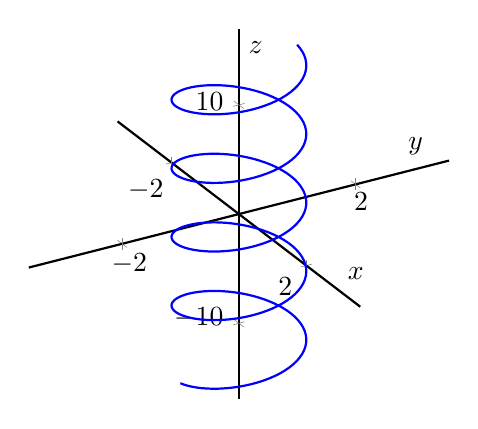
\begin{tikzpicture}
                            \begin{axis}[
                                width = 10cm,   % Ajusta el ancho total
                                height = 10cm,  % Ajusta el alto total
                                % --- CONFIGURACIÓN DE LA VISTA 3D ---
                                view={60}{30},            % Ángulo de cámara {azimut}{elevación}
                                axis lines = center,      % Ejes cruzándose en el origen
                                axis line style={-, thick}, % Ejes gruesos y con flecha (como pediste antes)
                                xlabel = {$x$},
                                ylabel = {$y$},
                                zlabel = {$z$},           % ¡Añadimos la etiqueta para Z!
                                xmin = -3, xmax = 3,
                                ymin = -3, ymax = 3,
                                plot box ratio = 1 1 1, % Proporción de X, Y y Z.
                                grid = major,
                                enlargelimits = true,
                                trig format plots=rad,    % Usamos radianes
                                % --- DEFINICIÓN DE CONSTANTES ---
                                % Cambia los valores de 'a' y 'b' aquí mismo. 
                                % 'c' calcula el denominador automáticamente para no ensuciar el código.
                                declare function={
                                    a=1; 
                                    b=1; 
                                    c=sqrt(a^2+b^2);
                                }
                            ]
                            % --- DEFINICIÓN DE LA CURVA 3D ---
                            \addplot3 [
                                domain=-20:20, % Rango de 't' (lo he hecho amplio para ver varias vueltas)
                                samples=300,   % En 3D se necesitan bastantes puntos para que sea suave
                                samples y=0,   % Truco vital: Evita que LaTeX intente dibujar una superficie
                                variable=\t,
                                thick,
                                blue,           % Color de la hélice
                            ]
                            % LAS ECUACIONES
                            ({a*cos(\t/c)}, {a*sin(\t/c)}, {b*\t/c});
                            
                            \end{axis}
                        \end{tikzpicture}
                        \end{figure}
                        \fi

                        \item En otro caso ($ab<0$) se dice que la hélice es dextrógira.

                        \ifshowfigures
                        \begin{figure}[H]
                            \centering
                        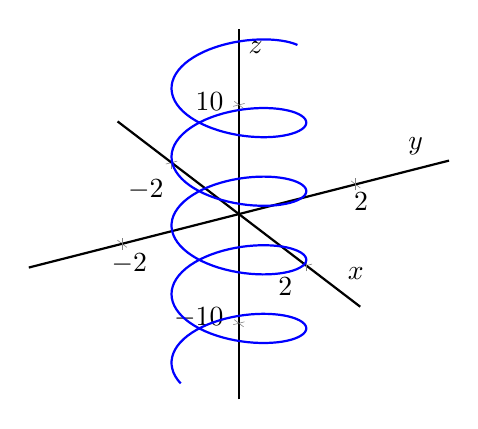
\begin{tikzpicture}
                            \begin{axis}[
                                width = 10cm,   % Ajusta el ancho total
                                height = 10cm,  % Ajusta el alto total
                                % --- CONFIGURACIÓN DE LA VISTA 3D ---
                                view={60}{30},            % Ángulo de cámara {azimut}{elevación}
                                axis lines = center,      % Ejes cruzándose en el origen
                                axis line style={-, thick}, % Ejes gruesos y con flecha (como pediste antes)
                                xlabel = {$x$},
                                ylabel = {$y$},
                                zlabel = {$z$},           % ¡Añadimos la etiqueta para Z!
                                xmin = -3, xmax = 3,
                                ymin = -3, ymax = 3,
                                plot box ratio = 1 1 1, % Proporción de X, Y y Z.
                                grid = major,
                                enlargelimits = true,
                                trig format plots=rad,    % Usamos radianes
                                % --- DEFINICIÓN DE CONSTANTES ---
                                % Cambia los valores de 'a' y 'b' aquí mismo. 
                                % 'c' calcula el denominador automáticamente para no ensuciar el código.
                                declare function={
                                    a=-1; 
                                    b=-1; 
                                    c=sqrt(a^2+b^2);
                                }
                            ]
                            % --- DEFINICIÓN DE LA CURVA 3D ---
                            \addplot3 [
                                domain=-20:20, % Rango de 't' (lo he hecho amplio para ver varias vueltas)
                                samples=300,   % En 3D se necesitan bastantes puntos para que sea suave
                                samples y=0,   % Truco vital: Evita que LaTeX intente dibujar una superficie
                                variable=\t,
                                thick,
                                blue,           % Color de la hélice
                            ]
                            % LAS ECUACIONES
                            ({a*cos(\t/c)}, {a*sin(\t/c)}, {b*\t/c});
                            
                            \end{axis}
                        \end{tikzpicture}
                        \end{figure}
                        \fi
                    \end{itemize}
            \end{itemize}

            \noindent
            Ahora, si $ab\neq 0$ veamos que la curva no es plana:

            \noindent
            Por reducción al absurdo, si fuera plana tendríamos que existe un plano $P\subset \mathbb{R}^3$ de forma que $\tr \theta\subset P$. Podemos tomar los puntos de la curva:
            \begin{align*}
                p_1 &= \theta(0) = (a, 0, 0) \\
                p_2 &= \theta\left(2\pi\sqrt{a^2+b^2}\right) = (a, 0, 2b\pi) \\
                p_3 &= \theta\left(\frac{\pi}{2}\sqrt{a^2+b^2}\right) = \left(0, a, \frac{\pi b}{2}\right) \\
                p_4 &= \theta\left(\pi \sqrt{a^2+b^2}\right) = (-a, 0, b\pi)
            \end{align*}
            Y como $\tr\theta\subset P$ tenemos por tanto que $p_1,p_2,p_3,p_4\in P$. Si consideramos los vectores:
            \begin{align*}
                v_1 &= p_2 - p_1 = (0, 0, 2b\pi) \\
                v_2 &= p_3 - p_1 = \left(-a, a, \frac{\pi b}{2}\right) \\
                v_3 &= p_4 - p_1 = (-2a, 0, b\pi)
            \end{align*}
            Observemos que:
            \begin{equation*}
                \left|\begin{array}{ccc}
                    0 & -a & -2a \\
                    0 & a & 0 \\
                    2b\pi & \nicefrac{\pi b}{2} & b\pi
                \end{array}\right| = 4a^2b\pi \neq 0
            \end{equation*}
            Por lo que $v_1,v_2,v_3$ son tres vectores contenidos en un plano que son linealmente independientes, \underline{contradicción}, que viene de suponer que $\theta$ es una curva plana.
    \end{enumerate}
\end{ejemplo}
